\onecolumn
\setcounter{equation}{0}
\renewcommand\theequation{A.\arabic{equation}}
\section*{A}
\label{sec:appendix}

  \[A =
    \mqty[b_1 & c_1 & 0 & \hdots & \hdots & 0 \\
          a_1 & b_2 & c_2 & 0 & \hdots & 0 \\
          0 & a_2 & b_3 & c_3 & \hdots & 0 \\
          \vdots & \ddots & \ddots & \ddots & \ddots & \vdots \\
          0 & \hdots & \ddots & a_{n-2} & b_{n-1} & c_{n-1} \\
          0 & \hdots & \hdots & 0 & a_{n-1} & b_n],
  \]

\begin{figure}[htbp]
	\centering
	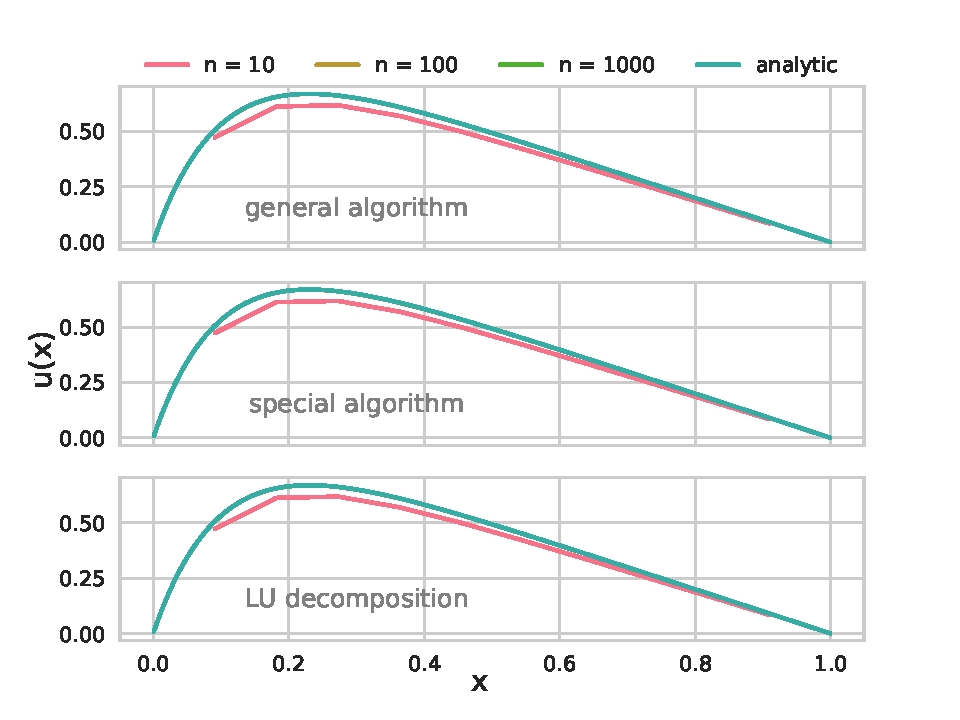
\includegraphics[width=\textwidth]{all_matrix_compare.pdf}
	\caption{The numeric solution using different solving algorithms. The graphs for n=100 and n=1000 are so similar that they are not distinguishable.}
	\label{fig:all}
\end{figure}
